\documentclass[tikz,border=2mm]{standalone} 
\usetikzlibrary{positioning, decorations.text}
\usepackage{garamondx}
\usepackage{xcolor}
\usepackage{varwidth}
\definecolor{darkolivegreen}{rgb}{0.33, 0.42, 0.18}
\definecolor{darkbyzantium}{rgb}{0.36, 0.22, 0.33}
\definecolor{darkelectricblue}{rgb}{0.33, 0.41, 0.47}
\definecolor{deepchestnut}{rgb}{0.73, 0.31, 0.28}

\begin{document}
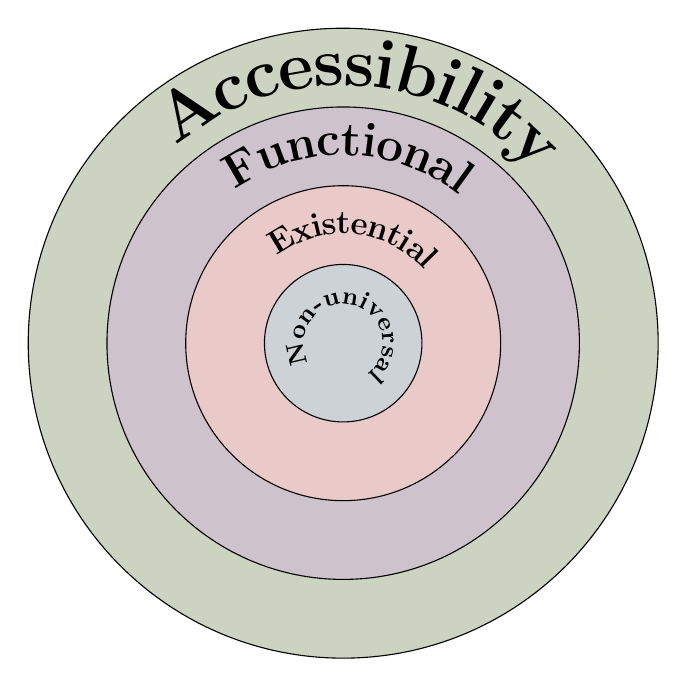
\begin{tikzpicture}

\node[circle, minimum size=8cm, draw, fill=darkolivegreen!30] (a) {};
\node[circle, minimum size=6cm, draw, fill=darkbyzantium!30] (b) {};
\node[circle, minimum size=4cm, draw, fill=deepchestnut!30] (c) {};
\node[circle, minimum size=2cm, draw, fill=darkelectricblue!30] (d) {};

\draw [decorate, decoration={text along path,raise=-1.5ex, text = {|\bfseries\scshape\Huge|Accessibility}}] (130:3.5) arc (130:0:3.5cm); 

\draw [decorate, decoration={text along path,raise=-0.75ex, text = {|\bfseries\scshape\LARGE|Functional}}] (125:2.5) arc (125:30:2.5cm); 

\draw [decorate, decoration={text along path,raise=-0.75ex, text = {|\bfseries\scshape\large|Existential}}] (127:1.5) arc (127:-90:1.5cm); 

\draw [decorate, decoration={text along path, text = {|\small\bfseries\scshape|Non-universal}}] (210:0.5) arc (210:-90:0.5cm); 

\end{tikzpicture}
\end{document}
